\section{方法}
\label{sec:method}

\subsection{问题定义与条件接口}
给定单视角 RGBA 图像 $I$，其有效前景记为 $F$，当前实现取 alpha 值大于 10 的像素。对应的生成资产记为 $\mathcal{G}$，用于三维推理的几何表示记为 $V$。目标是生成一张具有明确部件身份的二维引导图，并将其送入冻结的三维分割模型。图\ref{fig:method}展示整体流程，图\ref{fig:data}展示各引导分支的数据处理。本文将三类输出分开定义：二维整数标签图 $L$、英文部件记录 $\mathcal{A}$ 和下游三维分割输出 $\widehat{\mathcal{G}}$。它们分别回答“哪个像素属于哪个部件”“这个部件叫什么”以及“三维表面如何划分”。

在受控比较中，各条件应使用同一对象的输入渲染、生成资产和三维推理设置，而最终分割结果分别生成。该约束并不要求 A/B/C/D 的输出 GLB 相同，也不允许仅凭文件名认定输入一致。实际执行时需要对图像、GLB、VXZ 和模型配置分别保存指纹，并核验配对关系。原始下载资产仅作为数据来源，不能直接当作生成资产的逐面对应真值。

\begin{figure*}[t]
  \centering
  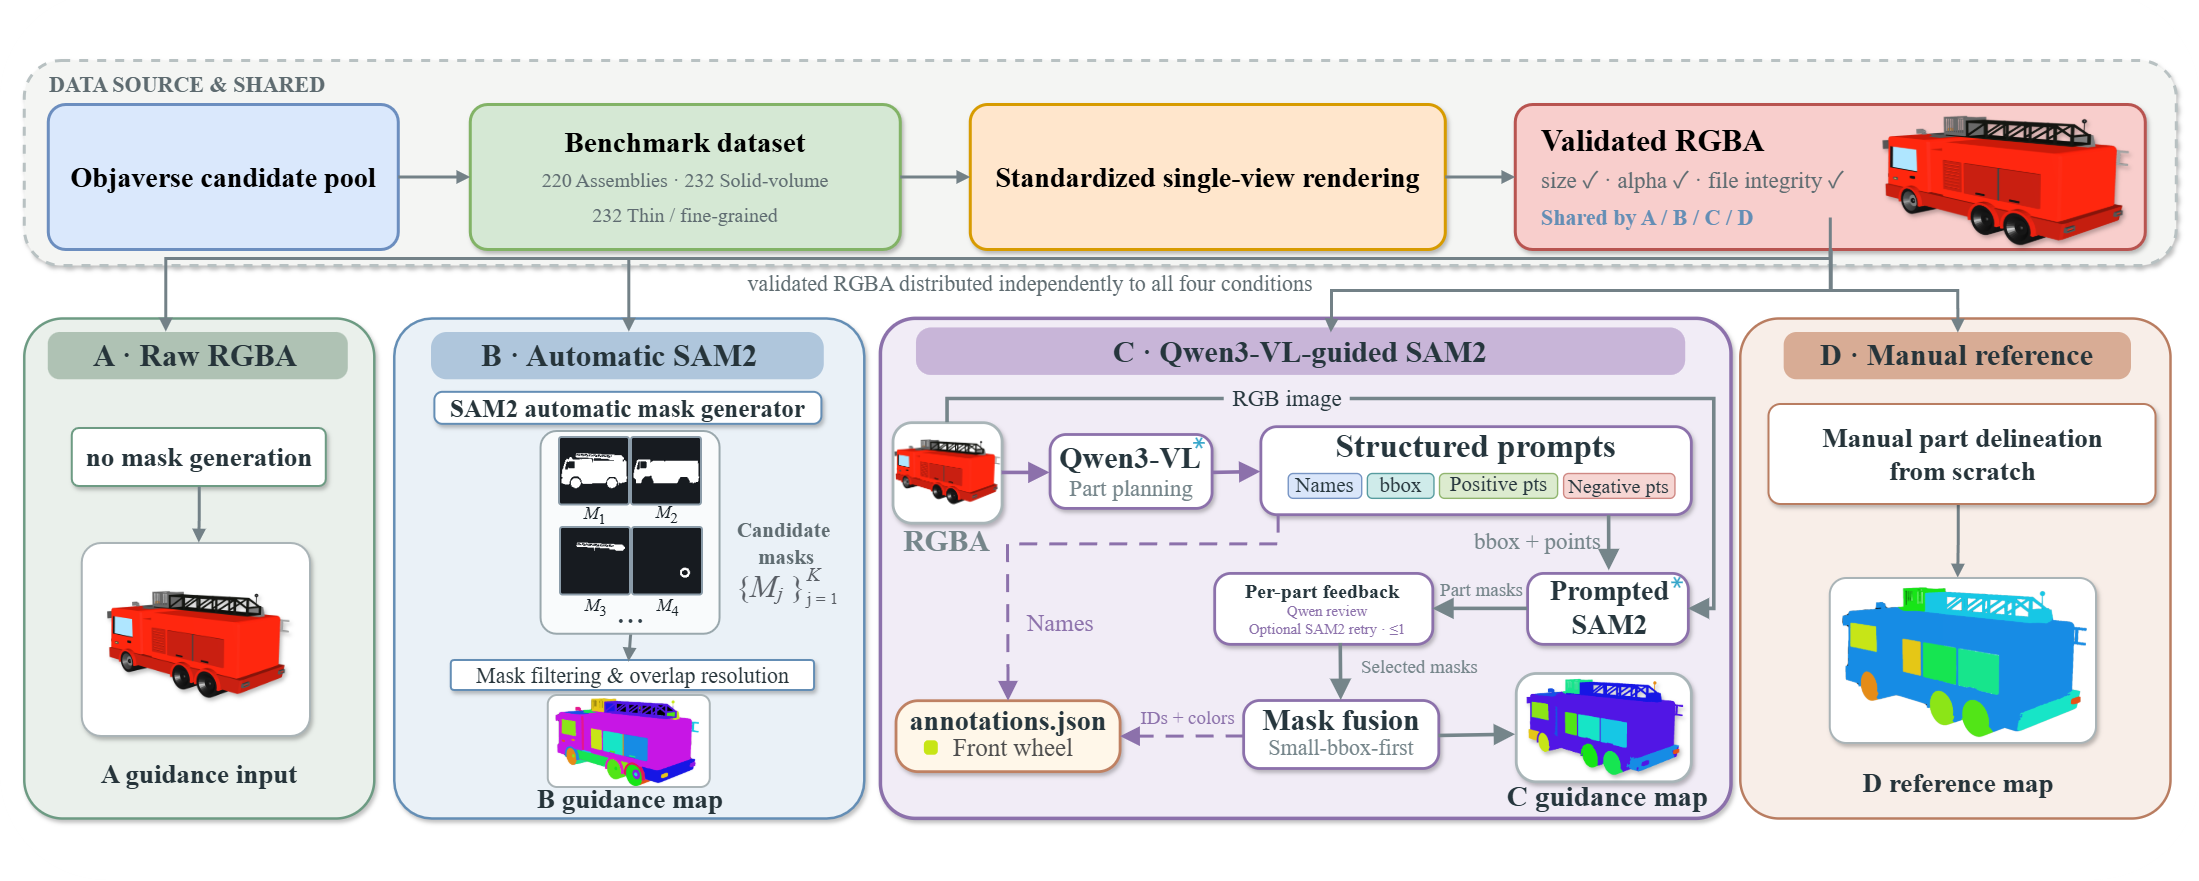
\includegraphics[width=\textwidth]{images/fig2_data.png}
  \caption{数据处理与四种引导条件。基准候选集按结构特征划分为 220 个组装结构、232 个实体体积结构和 232 个细薄／细粒度结构对象。A 使用原始 RGBA；B 从自动 SAM2 候选中筛选并处理重叠；C 使用部件规划、空间提示、候选反馈及小框优先融合，同时保存名称与二维标签的对应关系；D 为人工直接制作并渲染的二维部件参考，不来自 B 的自动结果修补，也不等同于完整三维真值。图内 D 的 ``from scratch'' 仅用于区别自动分支，具体人工制作流程仍需在数据说明中补全。C 的反馈在候选掩码阶段执行，每个被判为需要修正的候选至多重试一次。}
  \label{fig:data}
\end{figure*}


\subsection{可见部件规划与空间提示}
Qwen3-VL 接收 RGB 图像，输出可见部件的结构化记录集合
\begin{equation}
 \mathcal{R}=\{r_i\}_{i=1}^{K},\qquad
 r_i=(u_i,n_i,b_i,P_i^+,P_i^-),
 \label{eq:records}
\end{equation}
其中 $u_i$ 为候选部件编号，$n_i$ 为英文部件名称，$b_i$ 为边界框，$P_i^+$、$P_i^-$ 为正、负提示点。规划面向当前视角的可见结构；遮挡后方的部件不能仅凭类别常识被当作已观察到的区域。对于车轮、支架等重复实例，名称相同并不意味着实例相同，应结合位置保留独立记录。

框限制候选范围，正点指向目标内部，负点排除相邻结构。它们承担不同约束，不能以提示点更多推断分割一定更好。多个正点可能落在不同部件，负点也可能误落在目标上。本文以结构化记录为基础进行解析和坐标检查，再将有效空间提示传入 SAM2。当前原型采用 $[0,1000]$ 归一化坐标；横、纵坐标分别按图像宽、高转换并裁剪到有效范围。正点通过前景邻域检查取得有效位置；没有有效正点的候选不进入正常掩码生成流程。最终测试应固定输入缩放与坐标转换实现，以避免图像和提示使用不同分辨率。

对第 $i$ 个候选，初始掩码为
\begin{equation}
 M_i^{(0)}=S_{\theta}(I;b_i,P_i^+,P_i^-),
 \label{eq:sam}
\end{equation}
其中 $S_{\theta}$ 是冻结的 SAM2，采用单掩码输出。名称与候选编号随记录保留，但不输入 SAM2 的提示编码器。SAM2 输出的预测质量分数只用于描述模型对自身掩码的估计，不作为参考标签上的真实 IoU。

\begin{figure*}[t]
  \centering
  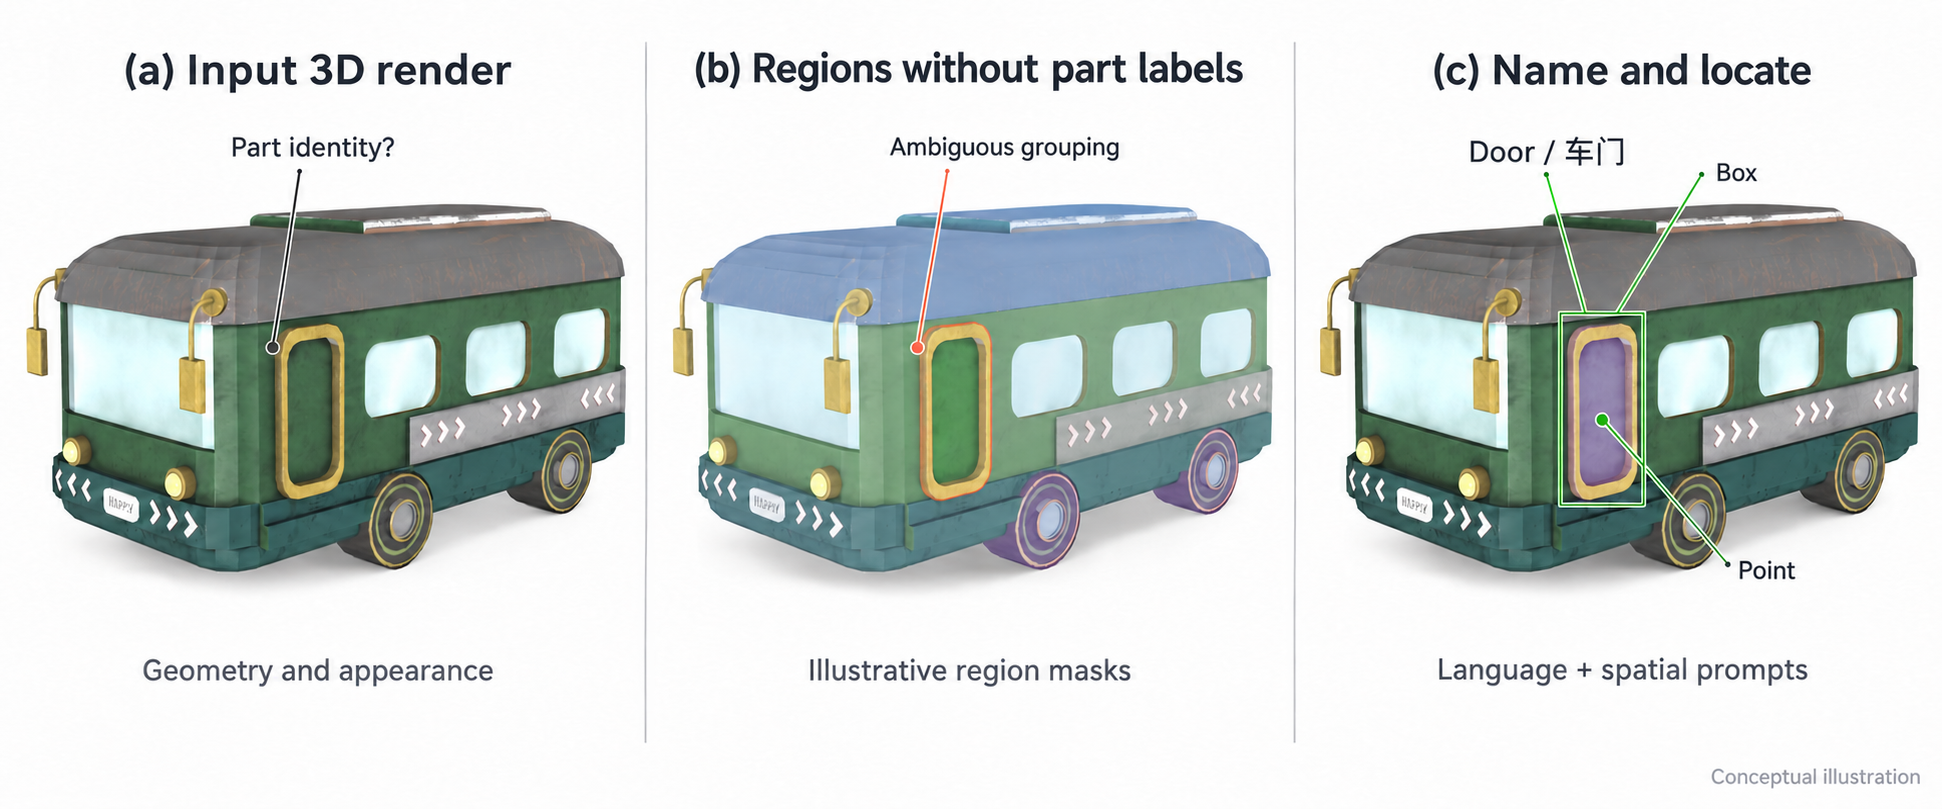
\includegraphics[width=\textwidth]{images/fig3_motivation.png}
  \caption{研究动机的概念示意。（a）三维渲染提供几何与外观，却未必提供可查询的部件名称；（b）无语义区域划分不能直接回答某一区域对应什么部件；（c）视觉语言模型将名称与框、点等空间提示关联，使分割目标具有明确的语义指向。该图为概念插图，不是 B/C 的实测对比，也不用于证明分割精度优越。}
  \label{fig:motivation}
\end{figure*}


\subsection{候选级视觉反馈}
仅靠首次规划，空间提示可能仍包含边界偏移、相邻部件干扰或重复区域。完整方法在融合之前对每个初始有效候选进行一次反馈判断。Qwen3-VL 查看原始 RGB、当前候选的红色掩码叠加图以及部件名称，判断掩码是否对应所述部件。反馈对象是单个候选，而非已经合成的整张彩色引导图；是否再次调用 SAM2 则由反馈结果决定。

若反馈认为候选需要修正，则保留已有提示，追加反馈点，并在可用时修正边界框，重新调用 SAM2：
\begin{equation}
 M_i^{(1)}=S_{\theta}(I;\widetilde b_i,
              P_i^+\cup\Delta P_i^+,P_i^-\cup\Delta P_i^-).
 \label{eq:feedback}
\end{equation}
每个候选至多重试一次；判断为合格、反馈解析失败或重试未得到有效掩码时，保留初始有效结果并记录相应状态。因此反馈的设计意图是用可见误差修正空间约束，而不是无限次尝试直到达到人工参考。推理阶段不访问 D 参考，也不使用参考分数挑选反馈结果。

当前实现仅将反馈选择后的掩码送入后续处理，融合排序仍读取原始规划的框，连通域锚点使用首轮经前景检查后的首个正点，而不是反馈新增点。这一区别会影响结果复现，不能在图中把它表述为“所有部件记录同步更新”。后续若修改该行为，应作为新版本单独记录，并与本版结果分开比较。

\subsection{点引导清理与小框优先融合}
候选之间可存在覆盖关系：车身掩码可能包含车门或连接件，先写入大掩码会使小部件失去可分配区域。本文将候选清理和覆盖仲裁分开处理。设反馈选择的掩码为 $M_i$，清理算子为 $\mathcal{C}$，则
\begin{equation}
 \overline M_i=\mathcal{C}(M_i\cap F;p_i),
 \label{eq:clean}
\end{equation}
其中 $p_i$ 是首轮经前景检查后的首个正点。清理先裁剪到前景，再依据点选择主连通区域；若该点不落在掩码内，则选择最近区域，没有锚点时选择最大区域。为保留同一部件可能存在的分离可见片段，实现还保留面积达到阈值的附属连通区域，而非无条件只取一个连通块。随后执行 $3\times3$ 椭圆结构元闭运算、前景裁剪、再次连通域筛选和小孔填充。阈值与具体顺序列于附录\ref{app:implementation}。

将候选按原始边界框面积升序排列；面积相同则按清理后面积及候选编号确定顺序。记排序为 $\pi$，初始已占用集合 $U_0=\varnothing$，依次计算
\begin{align}
 R_{\pi(t)}&=\overline M_{\pi(t)}\setminus U_{t-1},\\
 U_t&=U_{t-1}\cup R_{\pi(t)}\quad\text{（候选通过面积检查时）}.
 \label{eq:fusion}
\end{align}
通过检查的剩余区域获得独立标签，过小区域被淘汰，并保留淘汰原因。这里的优先级来自框面积，而非最终掩码面积或名称类别；小框优先有助于避免小件被先占用的大区域吞并，但错误的小框也可能抢占合理区域，其收益需要由消融实验判断。

融合后若前景仍有未分配像素，将其归于最近的已接受标签：
\begin{equation}
 L(x)=L\!\left(\arg\min_{y\in U}\|x-y\|_2\right),
 \quad x\in F\setminus U .
 \label{eq:residual}
\end{equation}
这一步只补齐已有标签的覆盖，不产生新部件，也不能恢复规划中遗漏的语义。若所有候选均无效，则显式记录失败，不以整物体单标签伪装成成功。前景外标签为 $0$，整数标签图以 16 位格式保存，避免从抗锯齿颜色反推二维真实标签。

\subsection{三维分割与英文记录}
根据固定调色板 $c$ 将标签图转换为二维引导 $G(x)=c(L(x))$。冻结的 SegViGen 以三维资产表示和二维条件执行推理，可抽象为
\begin{equation}
 \widehat{\mathcal{G}}_k=H_{\phi}(V,G_k;\xi),\qquad
 k\in\{A,B,C,D\},
 \label{eq:3d}
\end{equation}
其中 $\phi$ 是固定模型参数，$\xi$ 表示种子及视角等运行设置。A 使用原始 RGBA 作为对照条件，不声称其包含显式部件标签；B、C、D 分别提供自动、语言引导和人工参考图。共享 $V$ 是本文受控比较的要求，最终需以实际运行清单确认。各组输出可因推理及导出过程具有不同纹理或拓扑，评价不能默认存在逐面编号对应。

对于 C 组的每个接受部件，保存
\begin{equation}
 \mathcal{A}_{\ell}=(\ell,u_i,n_i,c_{\ell},\text{mask path}),
 \label{eq:annotation}
\end{equation}
其中 $\ell$ 是融合后二维标签编号，英文名称 $n_i$ 统一保存于 \texttt{label} 字段，数值身份保存在 \texttt{label\_id} 字段。该记录保持从规划名称到二维区域的显式关联。本文当前实现不将名称字符串写入生成隐变量，也不将其直接送入 SegViGen。空间提示改变二维分割，二维引导再影响三维输出，这是名称发挥间接作用的路径。

需要进一步区分彩色三维分区与持久语义绑定。要使查看器点击任意表面后可靠显示名称，还需保存从三维表面元素到 $\ell$ 的明确映射；仅存在彩色 GLB 和二维 JSON 不能证明这一步已经完成。本初稿已核验的 V5 实现范围为二维名称关联与引导图生成；三维分区作为独立下游接口描述，仍需以本版实际运行记录验证。三维显式 ID 导出和交互命名验证列为后续系统扩展，不作为已完成的实验结论。
